\section{Revenue \& Rewards}\label{sec:revenue}

\subsubsection*{What is Colony Revenue?}
A colony may sell goods and services in exchange for its tokens, in exchange for ether or in exchange for one of the whitelisted ERC20 tokens. Whenever a colony receives such payments, we say that the colony has earned \emph{revenue}.

Revenue is distinct from a colony's working capital. The latter is the sum of all tokens held by the colony for use in funding requests, i.e. the funds in the pot belonging to the colony-wide domain in the colony (see Section \ref{sec:finance}), while the former, revenue, has its own dedicated pot.

\subsubsection*{What are Colony Rewards?}
There is some expectation that some fraction of any Ether or other valuable tokens earned by the colony are paid out to their token holding members\footnote{Accounts holding both tokens and reputation in the colony}. Whenever a colony distributes a portion of earned revenue to its token holding members, we say that the colony is paying out \emph{rewards}.

It is expected that most of the revenue will \emph{not} go towards rewards, but towards replenishing the working capital.

\subsection{Processing Revenue}
Revenue accumulates in a dedicated revenue pot. In order to be processed, a user has to make a special transaction, triggering the revenue distribution process. This process distinguishes between a colony's own token on the one hand and Ether, CLNY and the whitelisted tokens on the other:

\subsubsection*{Revenue earned in a colony's own token}
When a colony earns back some of its \emph{own} tokens as revenue, the revenue distribution process transfers them directly to the working capital, where they become part of the general fund allocation system of regular and mandated funding proposals (Section \ref{sec:pots-and-fp}).

\subsubsection*{Revenue earned in other currencies}
When a colony earns Ether or other currencies as revenue, the revenue distribution system allocates some of them to be claimed as rewards. In particular, the special triggering transaction takes any such revenue that has accumulated since the last such transaction, and makes 90\% available to the colony as working capital, while the remaining 10\% is used to pay out rewards to users that hold both colony tokens and reputation in the colony. (The split can be changed - see Section \ref{subsec:chaning-the-reward-split}).

\begin{center}
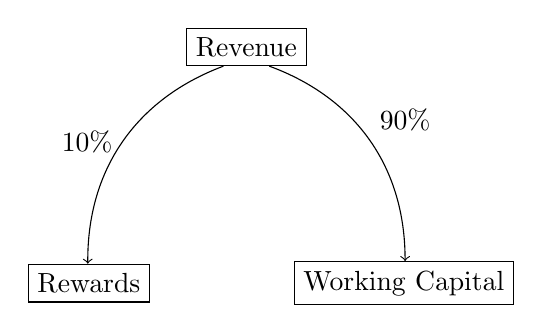
\begin{tikzpicture}
 
 \node[draw] at (-2,-3) (rewards) {Rewards};
 \node[draw] at (2,-3) (workingcapital) {Working Capital};
 \node[draw] at (0,0) (revenue) {Revenue}
    (revenue.-140) edge[bend right=35, ->] node[left]{10{\%}} (rewards)
    (revenue.-40) edge[bend left=35, ->] node[auto]{90{\%}} (workingcapital);
\end{tikzpicture}
\end{center}

\subsection{Claiming Rewards from the Reward Pot}\label{sec:claimrewards}
Rewards accumulate in the rewards pot. To trigger an actual payout to users (i.e. to make rewards claimable) a special type of proposal is made, proposing that all users should receive a payout based on the reward pot's holdings. 

This reward payout proposal includes the specific currency that should be paid, and only one currency is handled at a time. In the event that the proposal is approved by vote of reputation, then all user's tokens are locked until they claim their payout. Locking is necessary, because the token balance of each account factors into the rewards formula \eqref{eq:reward-claim}. Locking is triggered by incrementing the colony's `most recent payout' counter. 

Our currency contract contains a locking mechanism ensuring that a user cannot move tokens while they have votes to reveal; we use the same mechanism here to ensure that a user cannot move tokens after a payout is approved by the members of the colony but before the user has claimed their rewards. The colony has a counter for each user that is incremented whenever they claim a payout; they can also waive their claim to a payout that will increment this counter.  

While it is of course up to the members of each individual colony to decide, it is advisable that these payout proposals should only be accepted sporadically to keep the gas costs low for the users claiming their payouts, as well as simply to not be a nuisance to the users continually finding their tokens locked.

\textbf{Rewards are only available to accounts that hold both tokens and reputation}, and the amount claimable by each account depends on \emph{both} token balance and reputation (see equation \eqref{eq:reward-claim} below). Therefore we need to have a similar behaviour to `lock' the reputation of the users for the payout. When a payout is activated, the current state of the reputation tree is recorded in the payout itself. Users are paid out according to their reputation in this state, rather than the most recent state, to ensure all users get an appropriate payout and to avoid gaming the system (e.g. ``if I wait until I complete this task, I'll have more reputation and be able to claim more reward'').

\subsubsection*{The Rewards Formula}
The amount that each user ($u_i$) of a colony ($\mathcal{C}$) is entitled to claim ($p_i$) is a function of their colony token holdings ( $t_i$ ) and their total reputation in the colony ($r_i$).

\begin{equation}\label{eq:reward-claim}
 p_i = \left(\frac{t_i r_i}{T \times R}\right)^{\frac{1}{2}} \qquad \textnormal{where} \quad T = \sum\limits_{u_j\in \mathcal{C}} t_j \quad\textnormal{and}\quad R = \sum\limits_{u_j\in \mathcal{C}} r_j
\end{equation}

Note that this is very unlikely to payout all the tokens set aside for a payout - the only way it would do so is if everyone had the same proportion of reputation in the colony as they did proportion of tokens in the colony. However, the geometric average is the natural way to capture influence of two variables, and ensures that large token holders must earn large amounts of reputation to get the most from the payouts. The total tokens issued, total reputation and user reputation in the colony are all provable on-chain at claim time via a merkle proof that the \ascode{ReputationRootHash} (Section \ref{sec:reputationmining}) contains some values claimed by the user; the user's balance of colony tokens is trivial to lookup.

After some sufficiently long period of time (500000 blocks), all unclaimed tokens can be reclaimed by the colony and the payout closed. Any users that have not claimed their payout by that point will still have their tokens locked, and they will remain locked until they issue a transaction waiving their claim to the payout (indeed, they already passively did this by not claiming it in a timely fashion). Unclaimed tokens are returned to the reward pot and become part of the next reward cycle.


\subsubsection{Changing the split}\label{subsec:chaning-the-reward-split}

The 10\%/90\% split between rewards and capital can be altered based on a colony-wide vote of tokens and reputation. It requires a majority of both tokens and reputation in order to pass.




\subsection{The Revenue Model of the Colony Network}\label{sec:networkrevenue}
The Colony Network must be able to sustain itself. In particular, the \rc\ (in control of the colony network and reputation mining) maintains the contracts that underpin the network and develops new functionality for the network, the development of which needs to be paid for. Long term, the development and maintenance of the network (including the reputation system) needs to be financed by the network itself. 

\subsubsection{The Network Fee}\label{sec:networkfee}
We propose a fee that is levied on task payments made. When a user claims payment for a task they have done (Section \ref{sec:claiming-bounty}), some small fraction is paid to the network. 

\begin{center}
 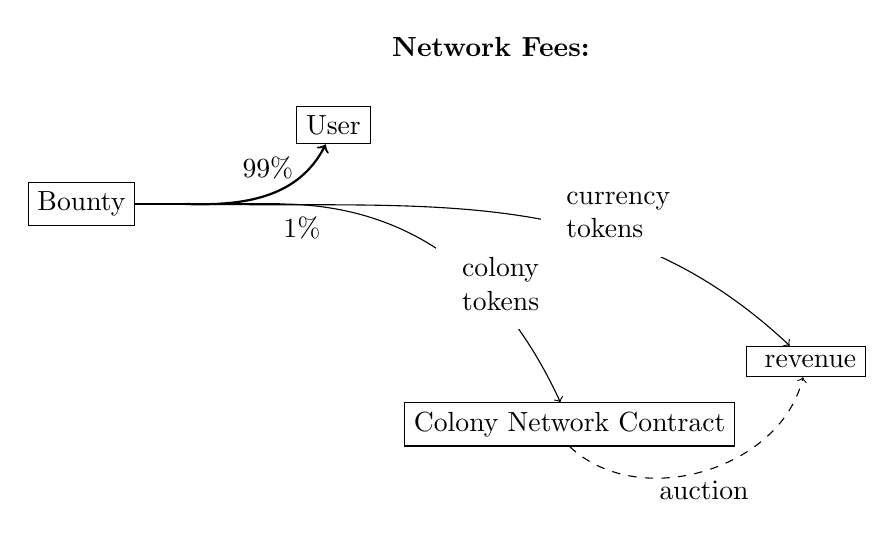
\begin{tikzpicture}
  \node at(0,2) {\textbf{Network Fees:}};
  \node at (-4,0) (dummy) {};
  \node[draw] at (-5.2,0) (bountybox) {Bounty};
  \node at (-2.8,0) (bounty) {}
   (bountybox.east) edge[-, thick] (dummy.east)
   (dummy.east) edge[-] (bounty.east);
   \node at (-2.4,-0.3) {{1\%}};
  \node[draw] at (-2,1) (user) {User};
  \node[draw] at (1,-2.8) (cnc) {Colony Network Contract};
  \node[draw] at (4,-2) (root) {\rc\ revenue}
    (dummy.east) edge[->, bend right=40,out=-25,thick] node[above=2pt] {99{\%}} (user) 
    (dummy.east) edge[->, bend left=30,out=12] node[fill=white,right=10pt] {\begin{tabular}{l} currency \\ tokens\end{tabular}} (root)
    (bounty.east) edge[->, bend left=30,out=35] node[fill=white, below right=-5pt] {\begin{tabular}{l} colony \\ tokens\end{tabular}} (cnc)
    (cnc.south) edge[->, bend right=60, dashed] node[below] {auction} (root)
    ;
 \end{tikzpicture}
\end{center}

The fees thus collected are sent to either the \rc\ (if the payment was in Ether or another whitelisted token) or the Colony Network Contract (if it was in a colony's token).


This idea of a fee is a little unusual for such a decentralised service. One reason why decentralised systems on Ethereum are appealing is that you don't have to pay a fee for the service, other than gas costs. However, we believe that the reputation system will ultimately be appealing enough that a small fee to pay for its existence will be acceptable.

The presence of a fee also means that we have to make some considerations that would be irrelevant to a more traditional decentralised system. For this reason, we will permission the read functions in the \ascode{EternalStorage} contract so that they can only be read by the Colony that owns the \ascode{EternalStorage} contract. This prevents a colony creating a contract that could be used to pay out Ether for tasks without paying the fee based on the status of tasks in the colony.

\subsubsection{The token auction}
The colony tokens collected are auctioned off by the Colony Network Contract, with the auctions denominated in \rcts, the proceeds of which are given to the \rc\ as revenue. These auctions - one for each type of token collected - occur on a regular basis of once a month.

We believe such behaviour would be beneficial for the \rcths\ (whose \rcts\ gain value by having an explicit use) and the \rc\ itself (which turns the fees into \rcts\ which it can then use to fund further development of the network without explicitly buying them back or creating more, diluting existing holders). It also provides an immediate mechanism of price discovery for the colony tokens, which are unlikely to be traded on third-party exchanges until much later in the lifetime of the colony. By auctioning off the collected tokens, we also prevent the \rc\ collecting a large number of different tokens that it has to manage, which would prove cumbersome and annoying for the colony.



